\documentclass[multi=tikzpicture,border=10pt]{standalone}
\usepackage{tikz}
\usepackage[compat=1.1.0]{tikz-feynman}

% ===== 字体：需要 XeLaTeX =====
\usepackage{fontspec}
\usepackage{xeCJK}
\usepackage{unicode-math}

% 正文
\setmainfont{Libertinus Serif}

% 数学
\setmathfont{Latin Modern Math}
\tikzset{
  source dot/.style={
    circle, fill=black, draw=black, inner sep=0pt, minimum size=5.5mm
  },
  blob/.style={
    circle, draw=black, thick, fill=white, inner sep=0pt, minimum size=12mm
  },
  blob with insertion/.style={
    circle, draw=black, thick, fill=white, inner sep=0pt, minimum size=12mm,
    path picture={
      \draw[black, thick]
      (path picture bounding box.north) -- (path picture bounding box.south);
    }
  }
}
\begin{document}






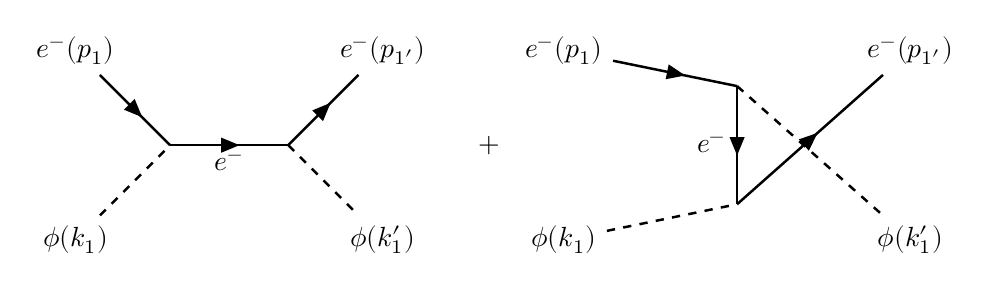
\begin{tikzpicture}[line width=0.9pt]

% Yukawa: e^- phi -> e^- phi, tree level
% first tree diagram
\begin{scope}[shift={(0,0)}]
  \begin{feynman}
    \vertex (iE) at (-1.2,  1.2) {$e^-(p_1)$};
    \vertex (iP) at (-1.2, -1.2) {$\phi(k_1)$};
    \vertex (vL) at ( 0.0,  0.0);
    \vertex (vR) at ( 1.5,  0.0);
    \vertex (fE) at ( 2.7,  1.2) {$e^-(p_{1'})$};
    \vertex (fP) at ( 2.7, -1.2) {$\phi(k_1')$};

    \diagram*{
      (iE) -- [fermion] (vL) -- [fermion, edge label'={$e^-$}] (vR) -- [fermion] (fE),
      (iP) -- [scalar]  (vL),
      (vR) -- [scalar]  (fP),
    };
  \end{feynman}
\end{scope}

\node at (4.05,0) {$+$};

% second tree diagram
\begin{scope}[shift={(7.2,0)}]
  \begin{feynman}
    \vertex (iE) at (-2.2,  1.2) {$e^-(p_1)$};
    \vertex (iP) at (-2.2, -1.2) {$\phi(k_1)$};
    \vertex (vT) at ( 0.0,  0.75);
    \vertex (vB) at ( 0.0, -0.75);
    \vertex (fE) at ( 2.2,  1.2) {$e^-(p_{1'})$};
    \vertex (fP) at ( 2.2, -1.2) {$\phi(k_1')$};

    \diagram*{
      (iE) -- [fermion] (vT) -- [fermion, edge label'={$e^-$}] (vB) -- [fermion] (fE),
      (iP) -- [scalar]  (vB),
      (vT) -- [scalar]  (fP),
    };
  \end{feynman}
\end{scope}

\end{tikzpicture}

\newpage
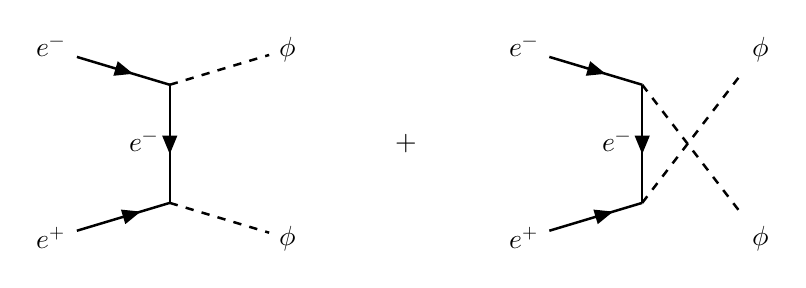
\begin{tikzpicture}[line width=0.9pt]


% e^- e^+ -> phi phi
\begin{scope}[shift={(0,0)}]
  \begin{feynman}
    \vertex (iE)  at (-1.5,  1.2) {$e^-$};
    \vertex (iP)  at (-1.5, -1.2) {$e^+$};
    \vertex (vT)  at ( 0.0,  0.75);
    \vertex (vB)  at ( 0.0, -0.75);
    \vertex (fP1) at ( 1.5,  1.2) {$\phi$};
    \vertex (fP2) at ( 1.5, -1.2) {$\phi$};

    \diagram*{
      (iE) -- [fermion] (vT) -- [fermion, edge label'={$e^-$}] (vB),
      (vB) -- [anti fermion] (iP),
      (vT)  -- [scalar]  (fP1),
      (vB)  -- [scalar]  (fP2),
    };
  \end{feynman}
\end{scope}

\node at (3.0,0) {$+$};

\begin{scope}[shift={(6.0,0)}]
  \begin{feynman}
    \vertex (iE)  at (-1.5,  1.2) {$e^-$};
    \vertex (iP)  at (-1.5, -1.2) {$e^+$};
    \vertex (vT)  at ( 0.0,  0.75);
    \vertex (vB)  at ( 0.0, -0.75);
    \vertex (fP1) at ( 1.5,  1.2) {$\phi$};
    \vertex (fP2) at ( 1.5, -1.2) {$\phi$};

    \diagram*{
      (iE) -- [fermion] (vT) -- [fermion, edge label'={$e^-$}] (vB),
      (vB) -- [anti fermion] (iP),
      (vT)  -- [scalar]  (fP2),
      (vB)  -- [scalar]  (fP1),
    };
  \end{feynman}
\end{scope}

\end{tikzpicture}

\newpage
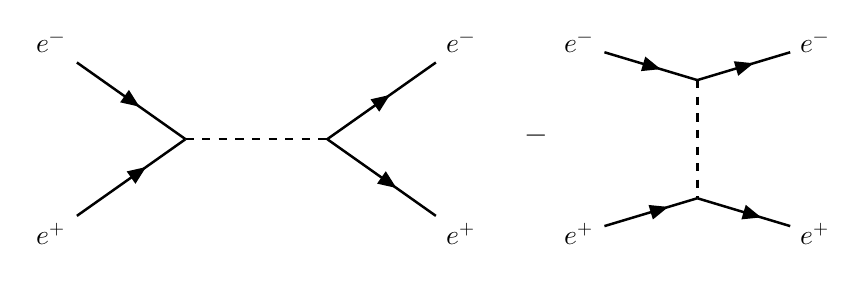
\begin{tikzpicture}[line width=0.9pt]

% e^- e^+ -> e^- e^+
\begin{scope}[shift={(0,0)}]
  \begin{feynman}
    \vertex (iE) at (-1.7,  1.2) {$e^-$};
    \vertex (iP) at (-1.7, -1.2) {$e^+$};
    \vertex (vL) at ( 0.0,  0.0);
    \vertex (vR) at ( 1.8,  0.0);
    \vertex (fE) at ( 3.5,  1.2) {$e^-$};
    \vertex (fP) at ( 3.5, -1.2) {$e^+$};

    \diagram*{
      (iE) -- [fermion]      (vL),
      (vL) -- [anti fermion] (iP),
      (vL) -- [scalar]       (vR),
      (vR) -- [fermion]      (fE),
      (fP) -- [anti fermion] (vR),
    };
  \end{feynman}
\end{scope}

\node at (4.45,0) {$-$};

\begin{scope}[shift={(6.5,0)}]
  \begin{feynman}
    \vertex (iE) at (-1.5,  1.2) {$e^-$};
    \vertex (iP) at (-1.5, -1.2) {$e^+$};
    \vertex (vT) at ( 0.0,  0.75);
    \vertex (vB) at ( 0.0, -0.75);
    \vertex (fE) at ( 1.5,  1.2) {$e^-$};
    \vertex (fP) at ( 1.5, -1.2) {$e^+$};

    \diagram*{
      (iE) -- [fermion]      (vT) -- [fermion]      (fE),
      (fP) -- [anti fermion] (vB) -- [anti fermion] (iP),
      (vT) -- [scalar]       (vB),
    };
  \end{feynman}
\end{scope}

\end{tikzpicture}

\newpage
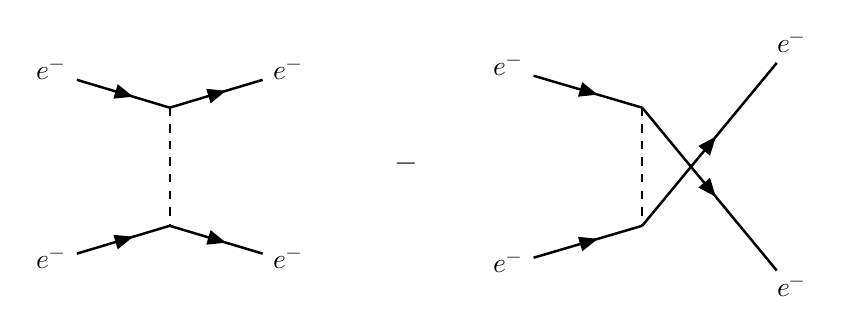
\begin{tikzpicture}[line width=0.9pt]

% e^- e^- -> e^- e^-
\begin{scope}[shift={(0,0)}]
  \begin{feynman}
    \vertex (iE1) at (-1.5,  1.2) {$e^-$};
    \vertex (iE2) at (-1.5, -1.2) {$e^-$};
    \vertex (vT)  at ( 0.0,  0.75);
    \vertex (vB)  at ( 0.0, -0.75);
    \vertex (fE1) at ( 1.5,  1.2) {$e^-$};
    \vertex (fE2) at ( 1.5, -1.2) {$e^-$};

    \diagram*{
      (iE1) -- [fermion] (vT) -- [fermion] (fE1),
      (iE2) -- [fermion] (vB) -- [fermion] (fE2),
      (vT)  -- [scalar]  (vB),
    };
  \end{feynman}
\end{scope}

\node at (3.0,0) {$-$};

\begin{scope}[shift={(6.0,0)}]
  \begin{feynman}
    \vertex (iE1) at (-1.7,  1.25) {$e^-$};
    \vertex (iE2) at (-1.7, -1.25) {$e^-$};
    \vertex (vT)  at ( 0.0,  0.75);
    \vertex (vB)  at ( 0.0, -0.75);
    \vertex (fE1) at ( 1.9,  1.55) {$e^-$};
    \vertex (fE2) at ( 1.9, -1.55) {$e^-$};

    \diagram*{
      (iE1) -- [fermion] (vT) -- [fermion] (fE2),
      (iE2) -- [fermion] (vB) -- [fermion] (fE1),
      (vT)  -- [scalar]  (vB),
    };
  \end{feynman}
\end{scope}

\end{tikzpicture}


\end{document}
